\chapter{SYSTEM ARCHITECTURE AND METHODOLOGY}

 
\vspace{10pt} % Adjust the value as needed

\section{Functional Requirement}

The functional requirements of the system are:
\begin{itemize}
  \item  To recognize and classify the Name Entities in any 
         given text documentation
  \item  To be able to precisely recognize and deal with the 
         Nepali language, aka     Devanagari text.
  \item  To analyze the data provided thoroughly and 
        efficiently with accuracy.
  \item To create a model for the Nepali language to identify 
        the words and determine Name Entities.
\end{itemize}

\section{System Development Tools}
\subsection{Google Colaboratory}
Colaboratory, or “Colab” for short, is a product from Google Research that allows anybody to write and execute arbitrary Python code through the browser. Colab is a hosted Jupyter Notebook service that requires no setup to use and provides free access to computing resources, including GPUs and TPUs. Colab is especially well suited to machine learning, data science, and education. \\
\\
We utilize Google Colab for our model development and training, simplifying our workflow by eliminating the need for code setup. With the availability of free GPU resources, accelerates and streamlines our model training processes, allowing us to efficiently save and manage our models on Google Drive \cite{colab}. 

\subsection{The Hugging Face Datasets Library}
The Hugging Face Datasets library provides a collection of high-quality datasets for natural language processing (NLP) and machine learning tasks. It simplifies the process of accessing and using various datasets, making it convenient for researchers and practitioners to experiment with different datasets for model development and evaluation.\\
\\
We use this library to import our .json data file from Google Drive into the code, utilizing the data for the subsequent training of our model \cite{HuggingFace}.

\subsection{Seqeval(Sequence Labeling Evaluation)} 

Seqeval is a Python library that can evaluate the performance of chunking tasks such as named-entity recognition, part-of-speech tagging, and semantic role labeling. It provides different metrics such as accuracy score, precision score, recall score, and f1-score to evaluate the performance of the model \cite{seqeval}.

\subsection{Weights and Biases (wandb)}
WandB is a powerful platform for monitoring and refining machine learning trials. It provides essential tools for users to easily monitor, display, and manage their experiments, designed for both researchers and developers. Widely used in deep learning, WandB is crucial for practitioners in neural network development. In our projects, it's essential for navigating and understanding the complexity of training and optimizing machine learning models \cite{W.}.

\section{Transformer}
The paper ‘Attention Is All You Need’ \cite{attention}  introduces a novel architecture called Transformer. As the title indicates, it uses attention. The attention-mechanism looks at an input sequence and decides at each step which other parts of the sequence are important. It sounds abstract but let us clarify with an easy example: When reading this text, you always focus on the word you read but at the same time your mind still holds the important keywords of the text in memory in order to provide context.\\
\\
An attention-mechanism works similarly for a given sequence. For our example with the human Encoder and Decoder, imagine that instead of only writing down the classification of the words in the imaginary language, the Encoder also writes down keywords that are important to the semantics of the sentence, and gives them to the Decoder in addition to the regular classification. Those new keywords make the classification much easier for the Decoder because it knows what parts of the sentence are important and which key terms give the sentence context \cite{Transformer?}.\\
\\
Transformer is an architecture for transforming one sequence into another one with the help of two parts (Encoder and Decoder), which is shown in [ Figure 3]. The Encoder is on the left and the Decoder is on the right. Both Encoder and Decoder are composed of modules that can be stacked on top of each other multiple times, which is described by Nx in the figure. We see that the modules consist mainly of Multi-Head Attention and Feed Forward layers. The inputs and outputs (target sentences) are first embedded into an n-dimensional space since we cannot use strings directly.\\
\\
One slight but important part of the model is the positional encoding of the different words. Since we have no recurrent networks that can remember how sequences are fed into a model, we need to somehow give every word/part in our sequence a relative position since a sequence depends on the order of its elements. These positions are added to the embedded representation (n-dimensional vector) of each word.   

% \begin{figure}[H]
% \centering
% \includegraphics[width=0.4\linewidth{img/Graphics/Transformer.png}
% \caption[ ]{The Transformer - model architecture}
% \label{fig: The Transformer - model architecture.png}

% \end{figure}

\begin{figure}[H]
\centering
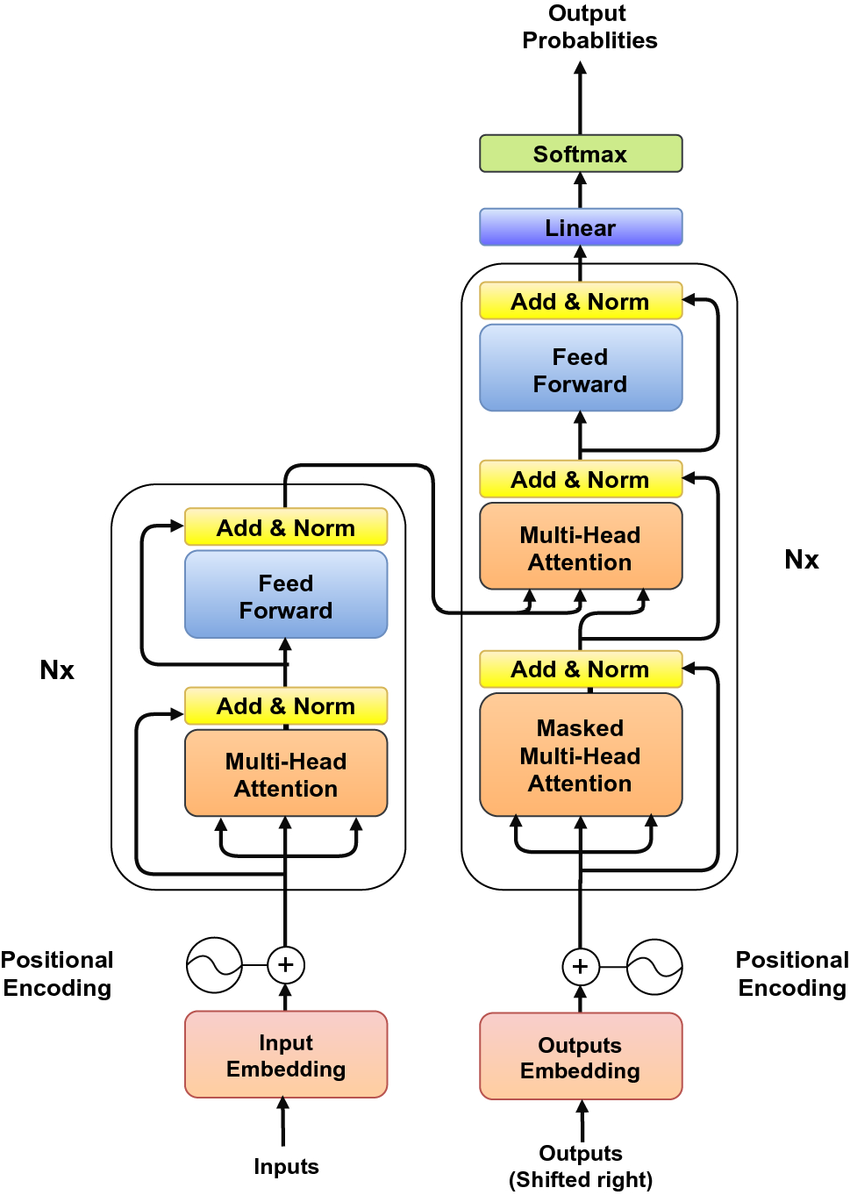
\includegraphics [scale=1.7]{img/Graphics/Transformer.png}
\caption[The Transformer – model architecture]{ The Transformer – model architecture \textit{(Source: \href{https://www.unite.ai/generative-ai-the-idea-behind-chatgpt-dall-e-midjourney-and-more/}{Unite.AI, 2024})}}
% \label{fig:DisplaCy.png}

\end{figure}

\newpage
Multi-Head Attention Bricks in the model:

\begin{figure}[H]
\centering
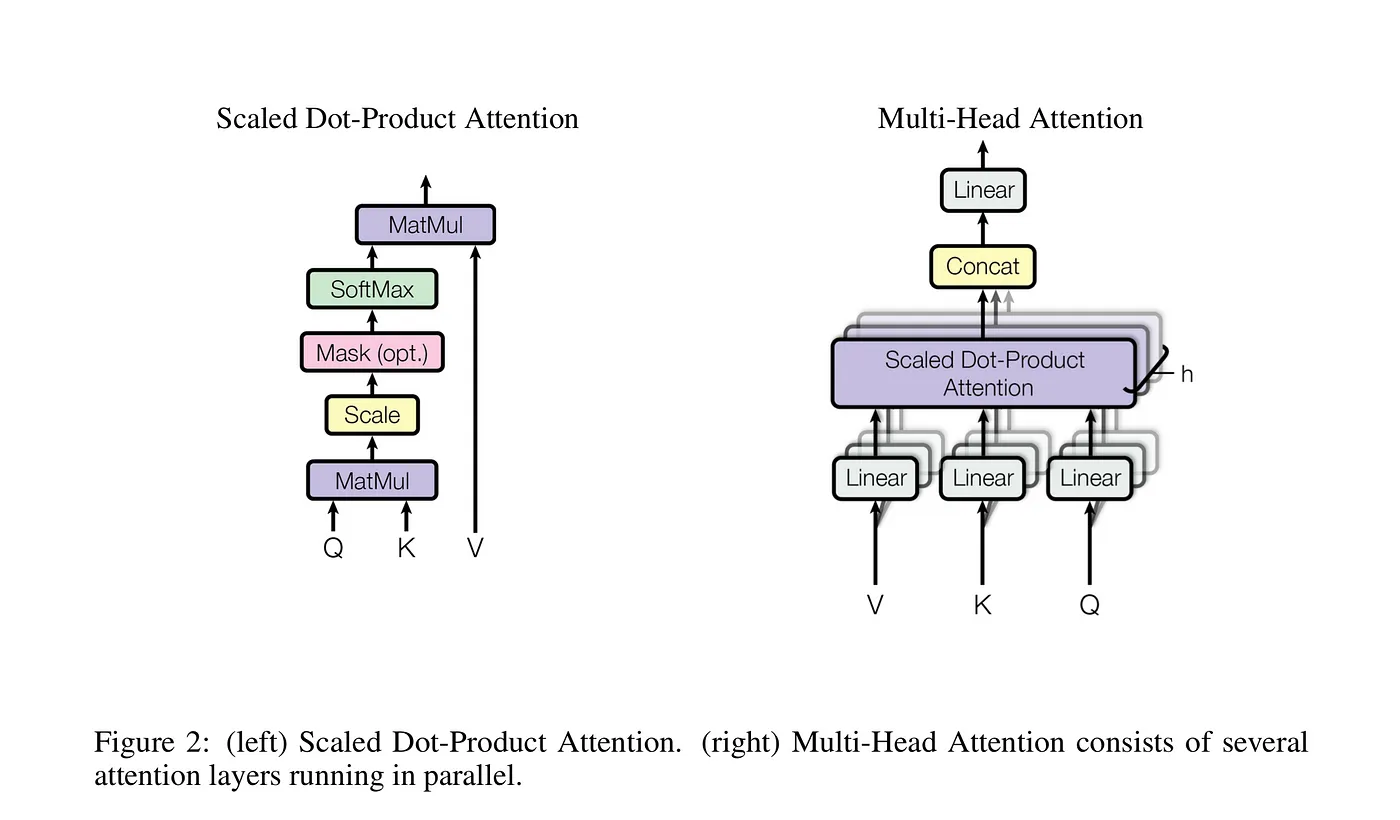
\includegraphics [scale=0.33]{img/transformer/transformer.png}
{\textit{(Picture Source: \href{https://medium.com/@tomiwaojo7910/decoding-the-transformer-architecture-revolutionizing-neural-networks-and-unveiling-components-61dedc49c24b}{Medium, 2024})}}
% \caption[ ]{  }
% \label{fig:DisplaCy.png}

\end{figure}


Left description of the attention mechanism. It’s not very complicated and can be described by the following equation:
\begin{equation}
\text{Attention}(Q, K, V) = \text{softmax}\left(\frac{QK^T}{\sqrt{d_k}}\right) V
\end{equation}


% \begin{figure}[H]
% \centering
% 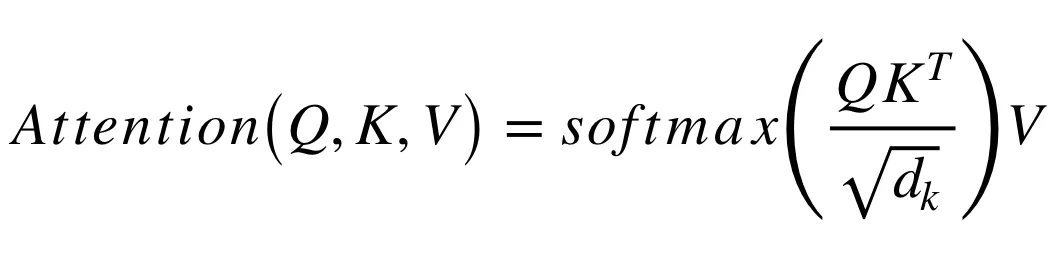
\includegraphics [scale=0.3]{img/transformer/f1.png}
% % \caption[ ]{  }
% % \label{fig:DisplaCy.png}

% \end{figure}


Q is a matrix that contains the query (vector representation of one word in the sequence), K are all the keys (vector representations of all the words in the sequence) and V are the values, which are again the vector representations of all the words in the sequence. For the encoder and decoder, multi-head attention modules, V consists of the same word sequence than Q. However, for the attention module that is taking into account the encoder and the decoder sequences, V is different from the sequence represented by Q.

To simplify this a little bit, we could say that the values in V are multiplied and summed with some attention-weights a, where our weights are defined by:

\begin{equation}
a = \text{softmax}\left(\frac{QK^T}{\sqrt{d_k}}\right)
\end{equation}

% \begin{figure}[H]
% \centering
% 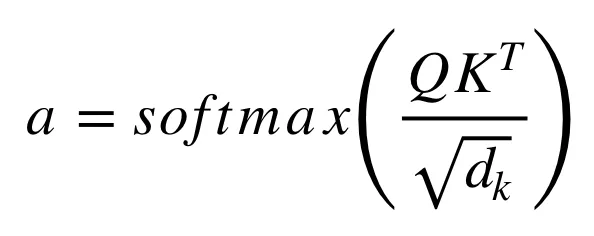
\includegraphics [scale=0.3]{img/transformer/f2.png}
% % \caption[ ]{ The Transformer – model architecture}
% % \label{fig:DisplaCy.png}

% \end{figure}

This means that the weights a are defined by how each word of the sequence (represented by Q) is influenced by all the other words in the sequence (represented by K). Additionally, the SoftMax function is applied to the weights a to have a distribution between 0 and 1. Those weights are then applied to all the words in the sequence that are introduced in V (same vectors than Q for encoder and decoder but different for the module that has encoder and decoder inputs).

The righthand picture describes how this attention-mechanism can be parallelized into multiple mechanisms that can be used side by side. The attention mechanism is repeated multiple times with linear projections of Q, K and V. This allows the system to learn from different representations of Q, K and V, which is beneficial to the model. These linear representations are done by multiplying Q, K and V by weight matrices W that are learned during the training.

Those matrices Q, K and V are different for each position of the attention modules in the structure depending on whether they are in the encoder, decoder or in-between encoder and decoder. The reason is that we want to attend on either the whole encoder input sequence or a part of the decoder input sequence. The multi-head attention module that connects the encoder and decoder will make sure that the encoder input-sequence is taken into account together with the decoder input-sequence up to a given position.

After the multi-attention heads in both the encoder and decoder, we have a pointwise feed-forward layer. This little feed-forward network has identical parameters for each position, which can be described as a separate, identical linear transformation of each element from the given sequence.

### Mathematical Example:

Suppose we have the following matrices for a transformer model:

\[ Q = \begin{bmatrix} 1 & 2 & 3 \\ 4 & 5 & 6 \end{bmatrix} \]

\[ K = \begin{bmatrix} 0 & 1 & 0 \\ 1 & 0 & 1 \end{bmatrix} \]

\[ V = \begin{bmatrix} 0 & 1 & 0 \\ 1 & 1 & 0 \end{bmatrix} \]

We want to compute the attention mechanism using the formula:

\[ \text{Attention}(Q, K, V) = \text{softmax}\left(\frac{QK^T}{\sqrt{d_k}}\right)V \]

1. Compute \( QK^T \):

\[ QK^T = \begin{bmatrix} 1 & 2 & 3 \\ 4 & 5 & 6 \end{bmatrix} \begin{bmatrix} 0 & 1 \\ 1 & 0 \\ 0 & 1 \end{bmatrix} = \begin{bmatrix} 2 & 1 \\ 5 & 4 \end{bmatrix} \]

2. Divide by \( \sqrt{d_k} \):

\[ \frac{QK^T}{\sqrt{d_k}} = \frac{1}{\sqrt{3}} \begin{bmatrix} 2 & 1 \\ 5 & 4 \end{bmatrix} \approx \begin{bmatrix} 1.155 & 0.577 \\ 2.887 & 2.31 \end{bmatrix} \]

3. Apply softmax:

\[ \text{softmax}\left(\frac{QK^T}{\sqrt{d_k}}\right) = \begin{bmatrix} 0.339 & 0.160 \\ 0.421 & 0.421 \end{bmatrix} \]

4. Multiply by \( V \):

\[ \text{Attention}(Q, K, V) = \begin{bmatrix} 0.339 & 0.160 \\ 0.421 & 0.421 \end{bmatrix} \begin{bmatrix} 0 & 1 & 0 \\ 1 & 1 & 0 \end{bmatrix} = \begin{bmatrix} 0.160 & 0.339 & 0.160 \\ 0.842 & 0.842 & 0.421 \end{bmatrix} \]

### NER Example:

Suppose we have the sentence: "Sara lives in New York City."

- Word embeddings for the sentence:

\[ Q = \begin{bmatrix} \text{Sara} \\ \text{lives} \\ \text{in} \\ \text{New} \\ \text{York} \\ \text{City} \\ \end{bmatrix} \]

- Context words relevant for NER:

\[ K = \begin{bmatrix} \text{lives} \\ \text{in} \\ \text{New} \\ \text{York} \\ \text{City} \\ \text{.} \\ \end{bmatrix} \]

- Words associated with named entities:

\[ V = \begin{bmatrix} \text{New} \\ \text{York} \\ \text{City} \\ \end{bmatrix} \]

The attention mechanism computes attention scores based on the similarity between the query and key vectors. The resulting matrix indicates which words are more relevant for identifying named entities based on the given context.

For instance, the attention scores may indicate higher relevance for words like "New", "York", and "City" in relation to the context words "lives" and "in", suggesting that these words are more likely to be part of a named entity in the sentence.

This combined example demonstrates the mathematical computation of the attention mechanism and its application in named entity recognition, showcasing both the formula functionality and its real-world relevance.

\newpage 
\section{BERT}

BERT, which stands for Bidirectional Encoder Representations from Transformers, is a state-of-the-art language model developed by Google AI for natural language processing (NLP) tasks. It has achieved remarkable success in various NLP tasks, including named entity recognition (NER).\\
\\
The Transformer, was originally designed as a model to translate one language to another. If we repurpose it for a different task, we would likely need to retrain the whole model from scratch. Given the time it takes to train a Transformer model is enormous, we would like to have a solution that enables us to readily reuse the trained Transformer for many different tasks. BERT is such a model. It is an extension of the encoder part of a Transformer.\\
\\
A BERT model is trained using the masked language model (MLM) and next sentence prediction (NSP) simultaneously. In Masked Language Model, certain percentage of input tokens (typically 15\%) are masked and model is supposed to predict the same input text along with the correct token for the masked tokens.\\
\\
Named Entity Recognition is a subtask of information extraction that aims to identify and classify named entities in text into predefined categories such as person names, locations, organizations, dates, etc. It is a crucial component in many NLP applications, including question-answering, sentiment analysis, machine translation, and more.\\
\\
BERT, based on the Transformer architecture, introduced a breakthrough in NLP by capturing contextual word representations. Unlike previous models that relied on shallow word embeddings, BERT considers the entire context of a word by utilizing a deep bidirectional architecture.\cite{BERT}

\begin{figure}[H]
\centering
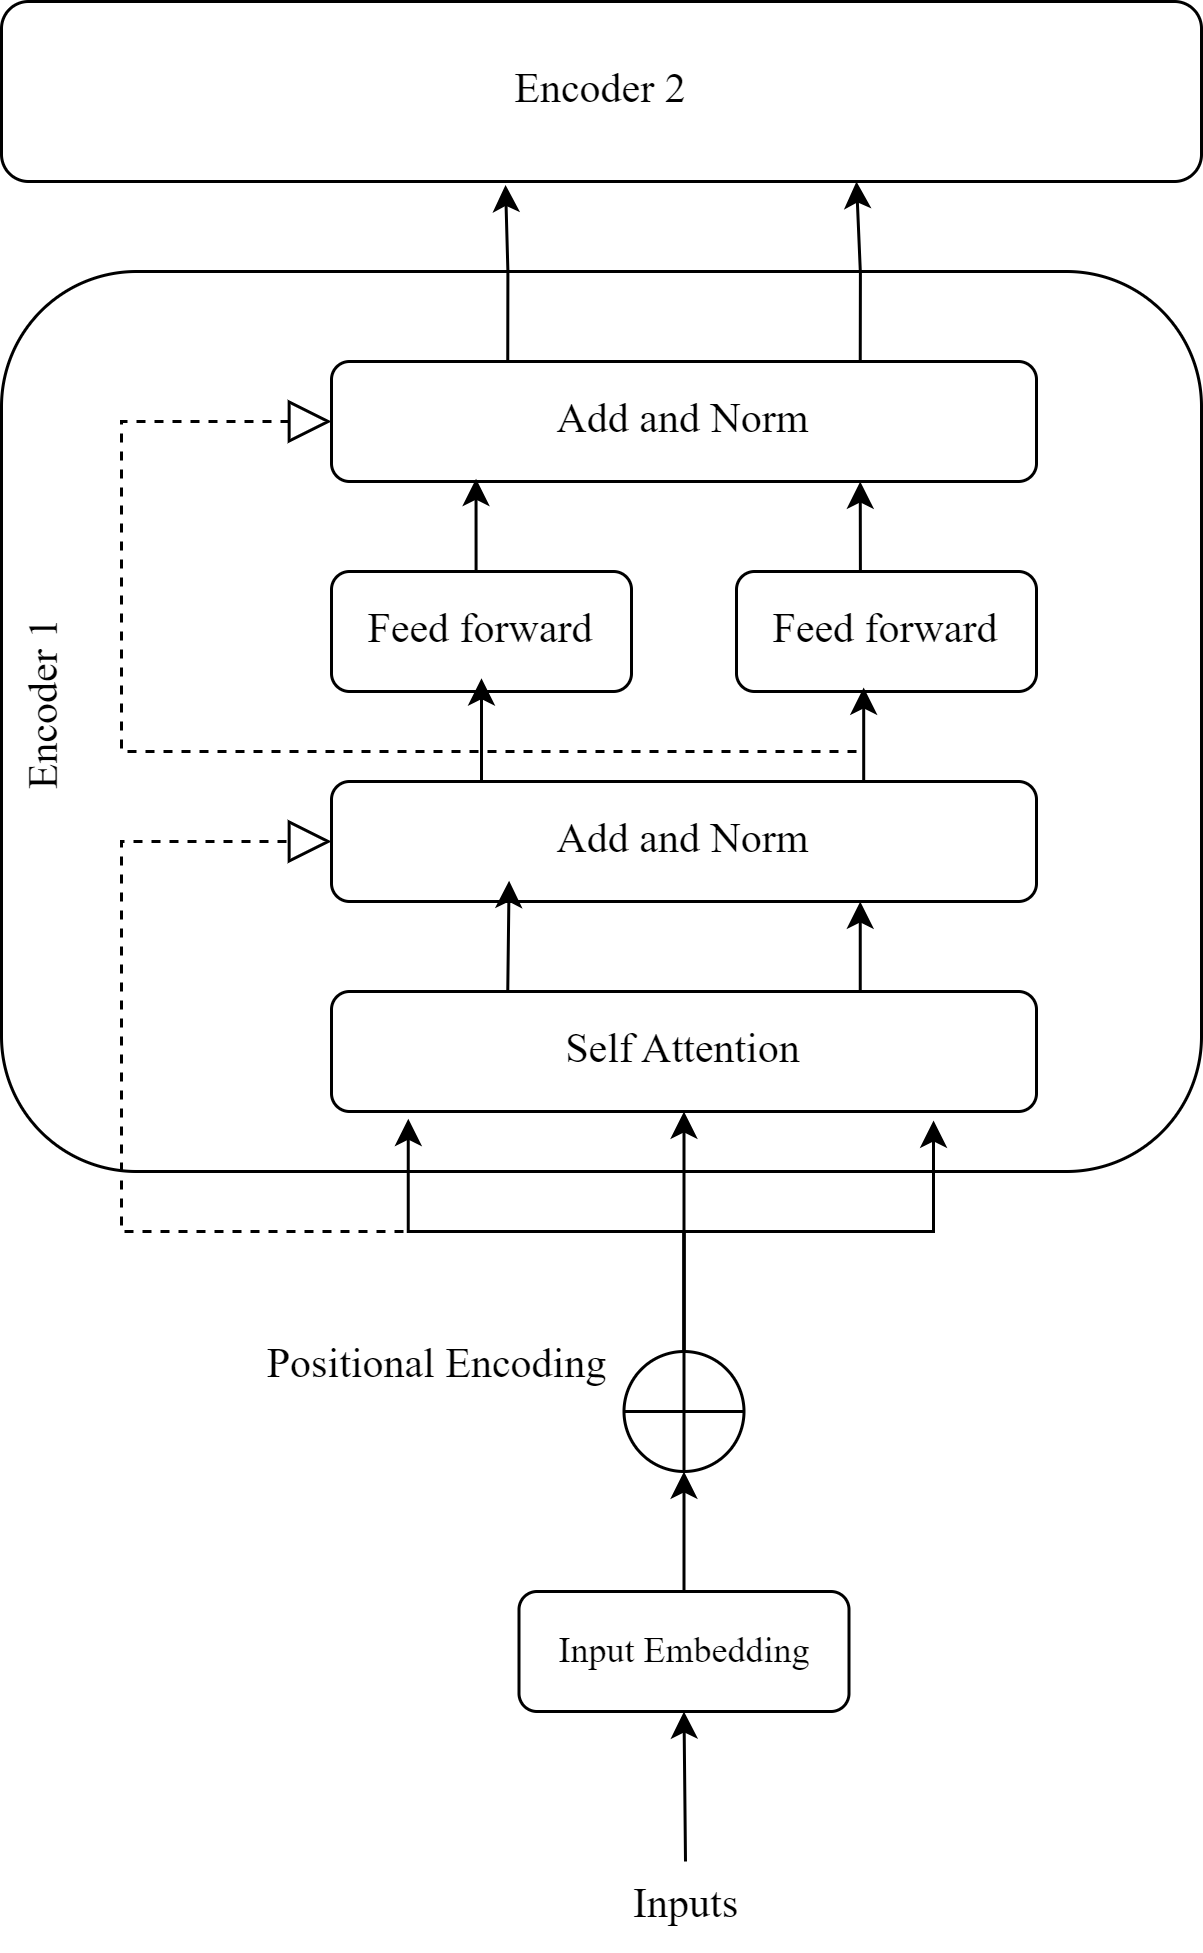
\includegraphics [scale=1.4]{img/Graphics/_Bert architecture.png}
\caption[ BERT Architecturee]{ BERT Architecture}
% \label{fig:DisplaCy.png}

\end{figure}


Here’s a brief overview of how BERT works for named entity recognition:
\begin{itemize}
    \item \textbf{The input embeddings} are the sum of the token embeddings, segment embeddings, and position embeddings. The position embedding encodes the absolute positions from 1 to the maximum sequence length (usually 512). At each position is a learnable embedding vector. Token embeddings are used to identify the word/subword being processed as input. Segment embeddings are the sentence number that is encoded into a vector. Position embeddings contain information about the relative position of a token in a sequence.
    \item \textbf{The self-attention} layer in the encoder module allows BERT to encode the context of each word from both directions, left and right.
    \item \textbf{Add and Norm} : In the Add step, it adds the layer's output to the input, helping with a problem called vanishing gradient. The Norm step is about making things consistent using layer normalization, which is another way of making the model work better. The point of Add \& Norm layers is to make training better without messing with the main part of the model.
    \item \textbf{Feed-Forward} : Each perceptron in one layer is connected to every perceptron on the next layer. Hence information is constantly "fed forward" from one layer to the next. The purpose of feedforward neural networks is to approximate functions.
\end{itemize}


 




% \newpage
% \section{Mathematical Modelling}
% \vspace{10pt} % Adjust the value as needed

% \subsection{Preprocessing}
% In our project, we utilized data from EVERESTner to classify Named Entities within sentences, encompassing 20,000 annotated sentences with labels such as B-Person, I-Person, B-Organization, I-Organization, B-Location, and I-Location. Originally in TXT format, this dataset was sourced from a GitHub repository. Concurrently, for model development, we drew insights from the WikiANN dataset, where meticulous data cleaning and preprocessing were imperative for training our SABDA-NER model. Each row in the WikiANN dataset contained 100 Nepali language sentences, and we seamlessly integrated this dataset into our training process.\\
% \\
% To further evaluate the model, we curated our own dataset for testing purposes, consisting of 1,700 manually annotated rows. This dataset serves to gauge the model's performance on novel and unseen data, allowing us to assess its generalization capabilities beyond the training data from EVERESTner and WikiANN.\\
% \\
% In the preprocessing phase, we initially converted our EVERESTner data into a CSV file, adhering to the specified annotation format. Subsequently, this data was transformed into a JSON file, aligning with the WikiANN structure, necessitating the use of "token\_set" and "ner\_tags" with numerical entity labels. String labels were replaced with numerical values, and after removing unnecessary columns, the formatted data was saved as a JSON file in our Google Drive.

% \subsection{Model Description}
% We developed our model using Google Colaboratory, leveraging the T4 GPU hardware accelerator. To load our data into Colab, we imported datasets from Hugging Face. Subsequently, we installed and imported the BERT tokenizer to tokenize Nepali language sentences and words. Further, we installed PyTorch. For evaluating the model's performance, we imported Seqeval to obtain score matrices, including accuracies and F1 scores.\\
% \\
% Our model was trained on the BERT-based-multilingual-cased architecture, chosen for its versatility across multiple languages. This model is widely used and reliable for custom data. Additionally, we incorporated W\&B (Weights \& Biases) for tracking machine learning work and training procedures, providing visualizations of model performance and scores.\\
% \\
% During training, we utilized the BERT-based-multilingual-cased model, specifying parameters such as 7 epochs, a learning rate of 2e-5, weight decay of 0.01, and logging steps at 1000. The training dataset comprised 16,000 sentences, with 4,700 sentences in the validation set. Utilizing the T4 GPU hardware accelerator, the training process took approximately 1 hour. Throughout training, accuracy scores increased, and training loss consistently decreased. The final model scores are presented in the following table.


% \begin{figure}[H]
% \centering
% 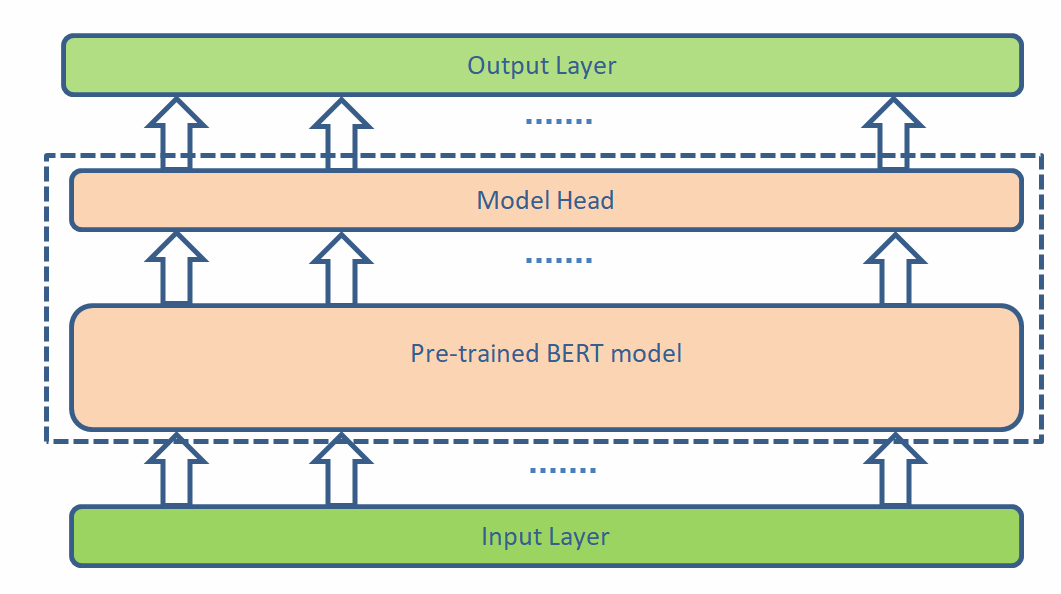
\includegraphics [scale=0.85]{img/Graphics/Model training Information.png}
% \caption[Model training Information]{ Model training Information}
% % \label{fig:DisplaCy.png}

% \end{figure}



% \begin{table}[H]
  
% \caption{Model training scores}
% \label{tab: Model training scores}
%     % \centering
    
%     % \begin{tabular}{|c|c|c|}
%     %     % \hline
%     %     % Column 1 & Column 2 & Column 3 \\
%     %     % \hline
%     %     % Row 1, Cell 1 & Row 1, Cell 2 & Row 1, Cell 3 \\
%     %     % Row 2, Cell 1 & Row 2, Cell 2 & Row 2, Cell 3 \\
%     %     % \hline
%     % \end{tabular}
    
    
% \end{table}

% \begin{figure}[H]
% \centering
% 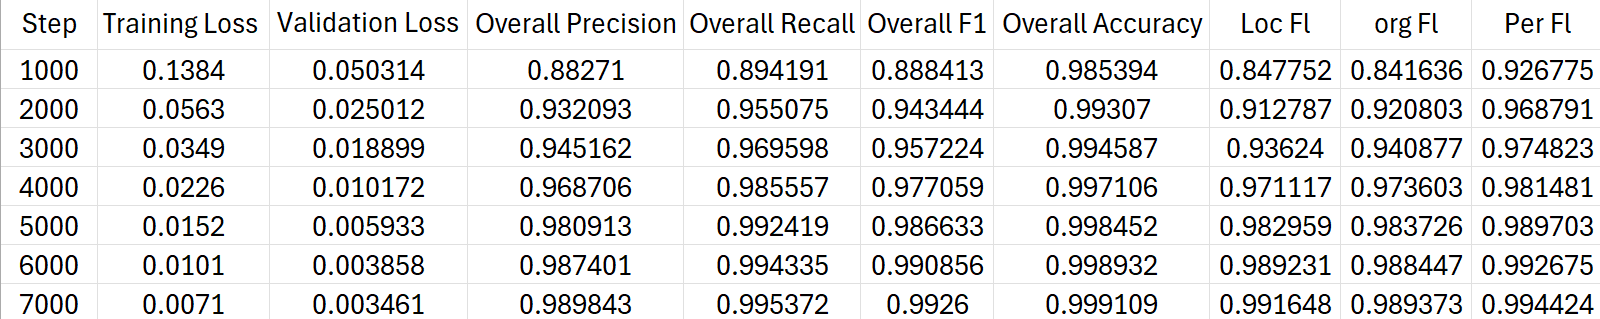
\includegraphics[width=\textwidth]{img/Graphics/Model training scores.png}

% \end{figure}



  
% We saved our model on Google Drive, enabling anyone with access to the model location to import and test results. Currently, testing involves manual sentence insertion, and we plan to extend this to test the entire dataset of 1,700 sentences at once for comprehensive evaluation. Initial scores are promising, and our next step is deploying the model on our website by uploading it to Hugging Face.

% \subsection{FastAPI}

% FASTAPI emerges as a crucial tool for deploying our NER model on the website. With FASTAPI, users can seamlessly interact with our model through the website's interface, enabling them to input sentences or links for information extraction via web scraping. This framework facilitates the smooth transfer of data from the user interface to the model, ensuring efficient processing of named entity classifications. The use of FASTAPI enhances the overall user experience, making it easy and reliable to obtain accurate results.

% \subsection{Web Scraping}
% Web scraping is a technique used to extract information from websites. It involves automatically fetching and parsing web page content to gather data, such as text, images, or links. Think of it as pulling useful information from a website's pages, making it accessible for various purposes, like analysis or integration into other applications. However, it's important to note that web scraping should be done ethically and in compliance with the website's terms of service.\\
% \\
% When deploying our model on the website, users can visit the site and input their sentences directly. Additionally, they have the option to insert a link on our website, allowing us to perform web scraping on the provided link. Our objective is to extract named entities, including persons, locations, and organizations, using our website. To access the web scraping procedure on the provided link, users need to navigate to the designated section on our website. Once initiated, the system will read all entities from the link and display the results on the screen of our website.





% \section{System Block Diagram}
% Must be accompanied by an explanation of the blocks and their interconnections
\newpage
\section{System Block Diagrams}
\vspace{20pt} % Adjust the value as needed

\subsection{System Architecture}
 


% The system for named entity recognition of nepali text involves two primary tasks. The first task is preparing the dataset and training 
% the BERT-based NER models. Once trained, the models are evaluated on test data to 
% obtain the final evaluation metrics. The model is then saved as binary files in HuggingFace, which is  
% used for generating the named entities .\\
% \\
%  The second task involves building a website that facilitates inferencing on user input and providing the information of SABDA-NER. Which is connected to HuggingFace SABDA-NER model through Fetch API which act as a middle man between website and model.

% The communication between the website and the remote server is facilitated by Fetch API.
% The web interface architecture enables users to get the result and input section where user can input nepali text. 

The named entity recognition (NER) system for Nepali text entails two primary tasks. In the initial phase, the focus is on preparing the dataset and conducting the training of BERT-based NER models. Following the training phase, these models undergo evaluation using test data to derive final performance metrics. Subsequently, the trained model is saved as binary files within the HuggingFace platform, a pivotal step that empowers the system to generate named entities based on Nepali text inputs.

Moving on to the second task, it involves the development of a website designed to streamline the process of inferencing on user-provided input while delivering information derived from the SABDA-NER model. This website establishes a seamless connection with the HuggingFace SABDA-NER model through the implementation of a Fetch API, strategically positioned as an intermediary that facilitates efficient communication between the website and the model.

The Fetch API expertly manages the communication dynamics between the website and the remote server. The architecture of the web interface is designed to empower users, providing a user-friendly experience by incorporating result presentation alongside a dedicated input section where users can input Nepali text for analysis and extraction of named entities.
 \begin{figure}[H]
\centering
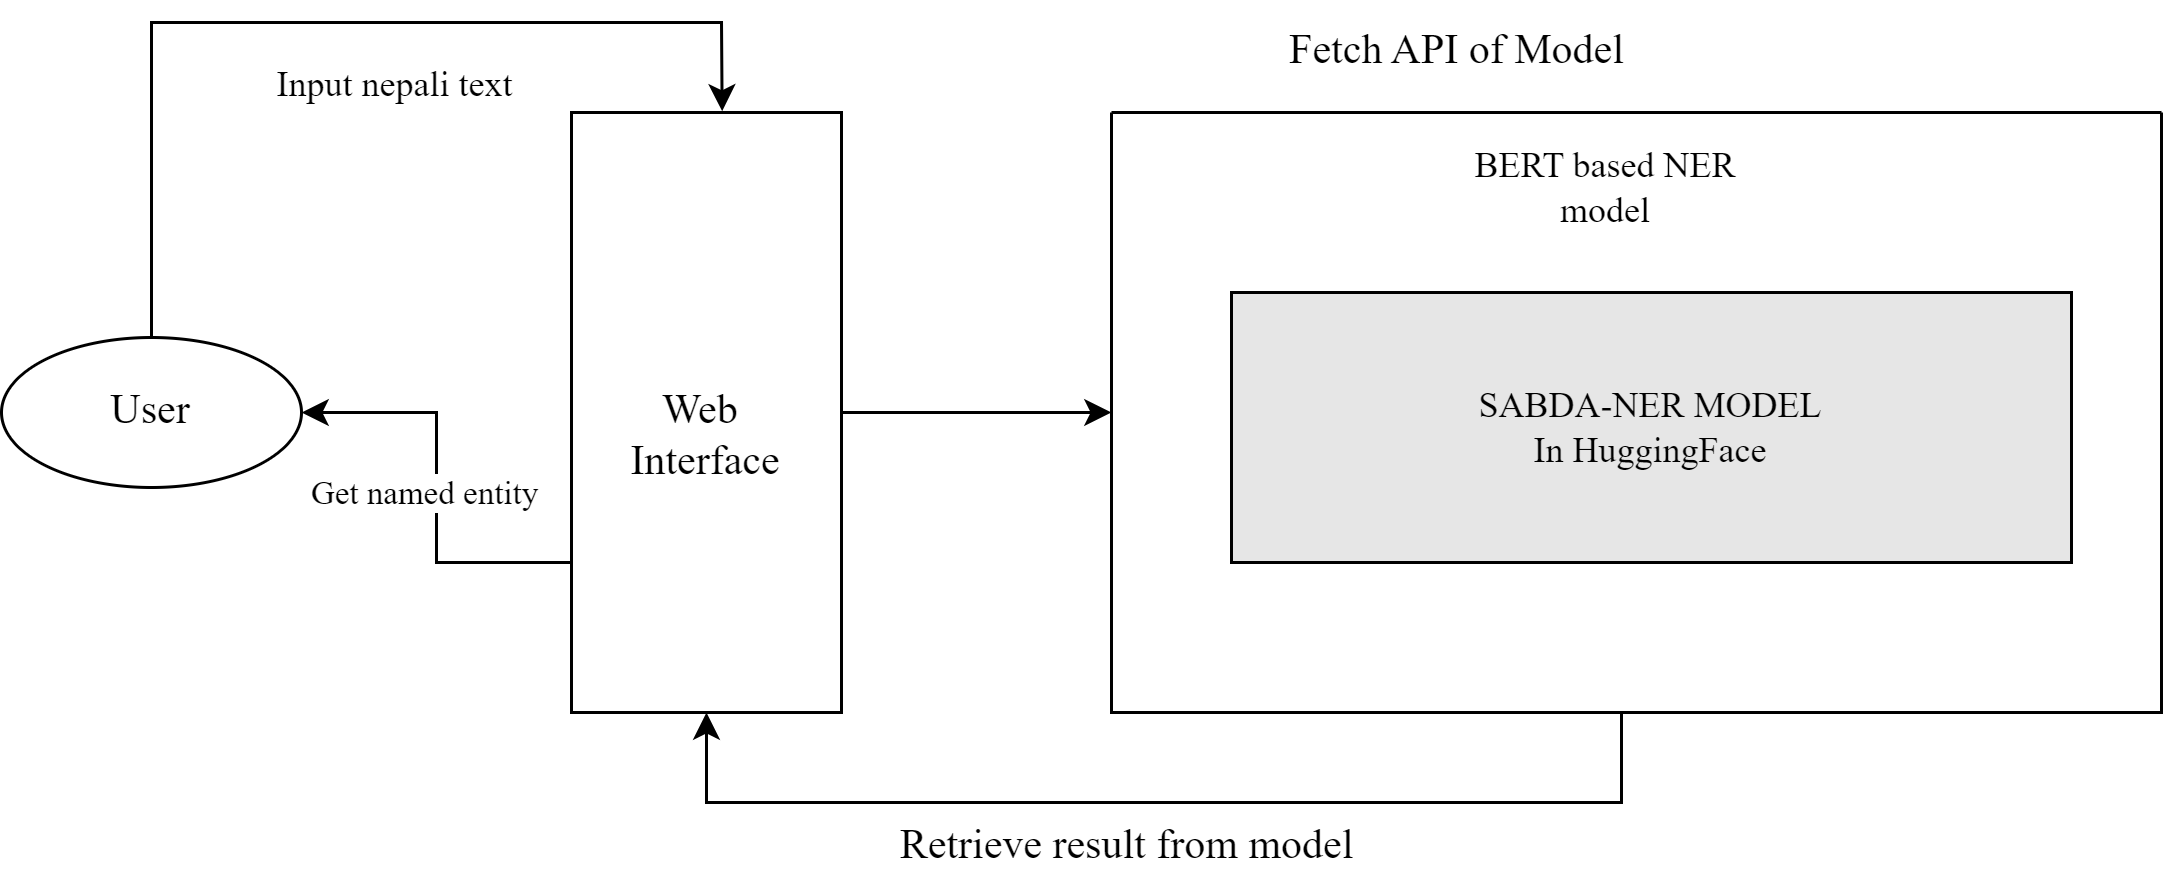
\includegraphics[scale=0.8]{img/systemBlock-etc/_NERsystemArchitecture.png}
\caption[ System Block diagram]{ System Block diagram}

\end{figure}


% \subsection{Model Architecture of Bidirectional Encoder Representations from Transformers (BERT)}

% \vspace{20pt}

%  \begin{figure}[H]
% \centering
% 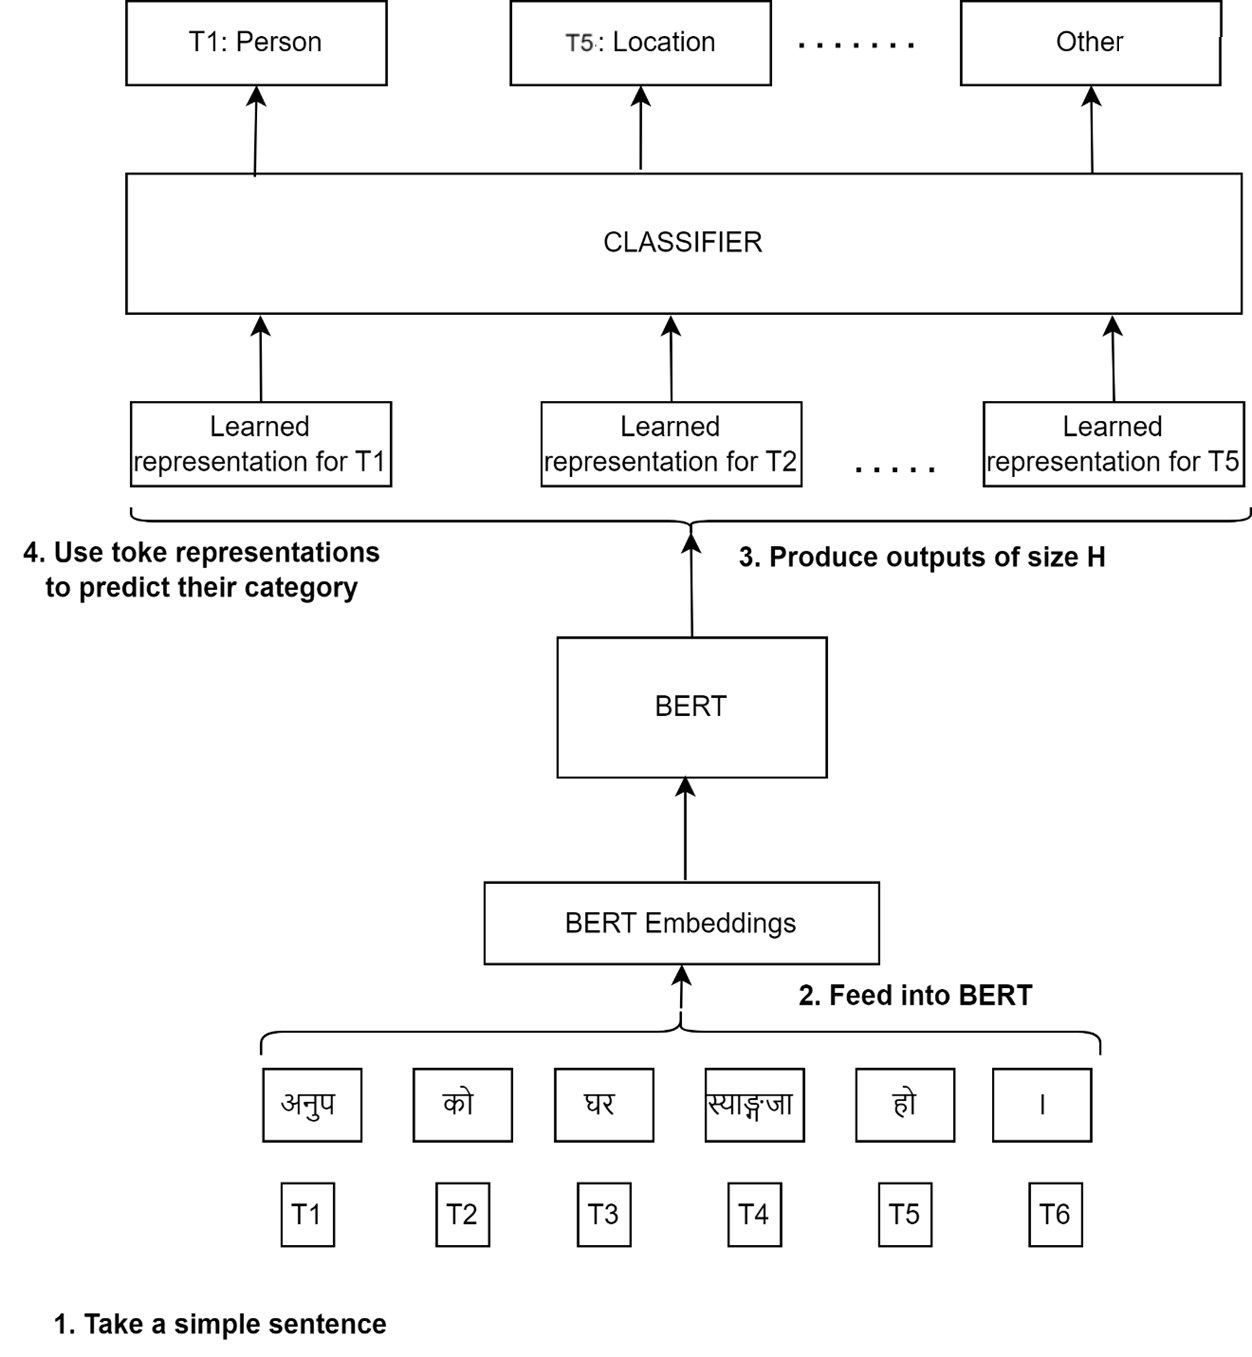
\includegraphics[width=1\textwidth]{img/systemBlock-etc/System Block diagram.png}
% \caption[ System Block diagram]{ System Block diagram}

% \end{figure}


%  \subsubsection {Input Stage}
% Input Text: The system takes raw text as input, which is the text to be analyzed for named entities.
% \subsubsection{Intermediate Stages}
% Tokenization and Embedding Layer: This stage involves tokenizing the input text into individual tokens and converting them into numerical embeddings using BERT's vocabulary. This layer also includes adding segment embeddings and positional encodings.
% \subsubsection{Multi-Head Self-Attention and Feedforward Layers}
% The token embeddings go through multiple layers of multi-head self-attention mechanisms and feedforward neural networks. This helps the model capture contextual relationships and create rich representations of the input tokens.
% \subsubsection{NER Classification Layers} 
% On top of the final hidden states, additional classification layers are added. These layers include fully connected networks followed by softmax activation. These layers predict the probability of each token belonging to different named entity classes (e.g., person, organization, location).
% \subsubsection{Output Stage}
% NER Predictions: The output of the NER classification layers provides predictions for each token's named entity label. Common labels include "B-PER" (beginning of a person entity), "I-PER" (inside a person entity), "B-ORG" (beginning of an organization entity), and so on.




\newpage
\subsection {Use Case Diagram}
\vspace{30pt} % Adjust the value as needed

 \begin{figure}[H]
\centering
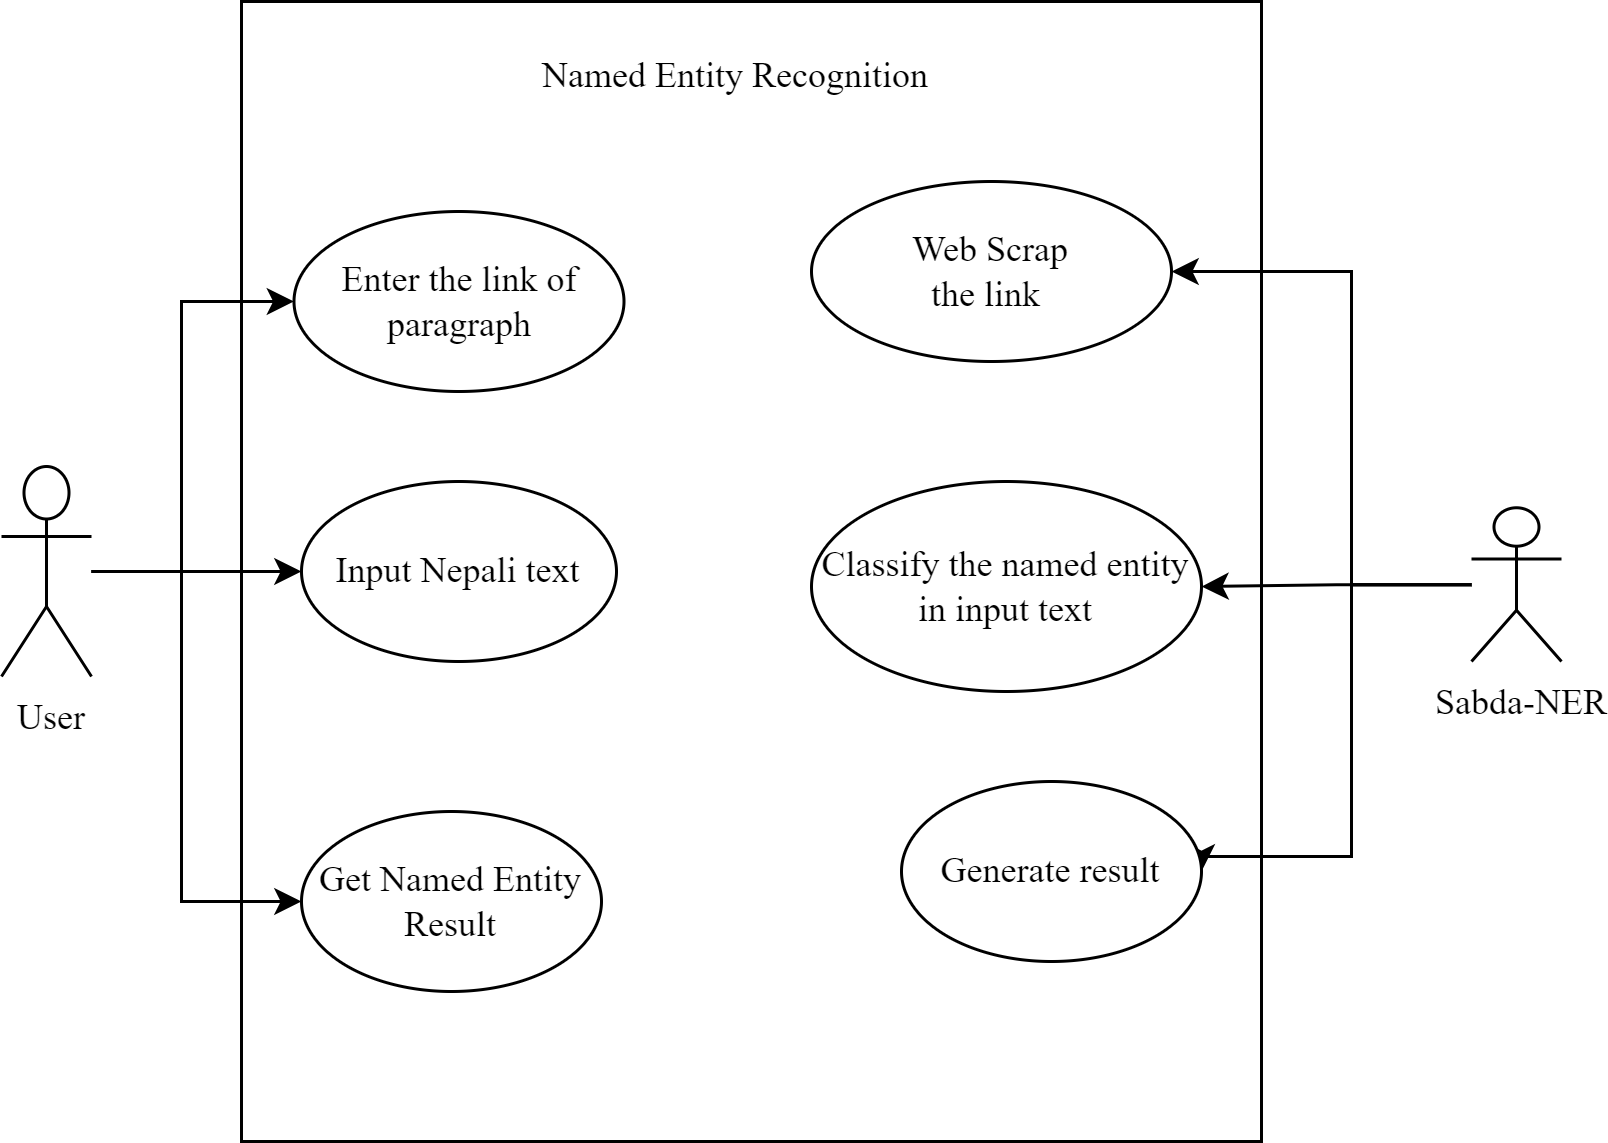
\includegraphics [scale=1.1]{img/systemBlock-etc/Use Case Diagram.png}
\caption[ Use Case Diagram]{ Use Case Diagram}
% \label{fig:DisplaCy.png}

\end{figure}

 
The use case diagram for our system illustrates various interactions and roles of the system’s users. The primary actors involved are the "User" and the "System". The User interacts with the system by uploading the Nepali text. The User can also access the system to view the named entity results of the entered text. On the other hand, the System is responsible for managing the system, including user authentication, system configuration, and monitoring the overall functionality. The use case diagram shows the main use cases, such as "data collection" "preprocessing", and "View classified Results" which represent the key functionalities of the system.



\subsection{Sequence Diagram} 
\vspace{30pt} % Adjust the value as needed

  \begin{figure}[H]
\centering
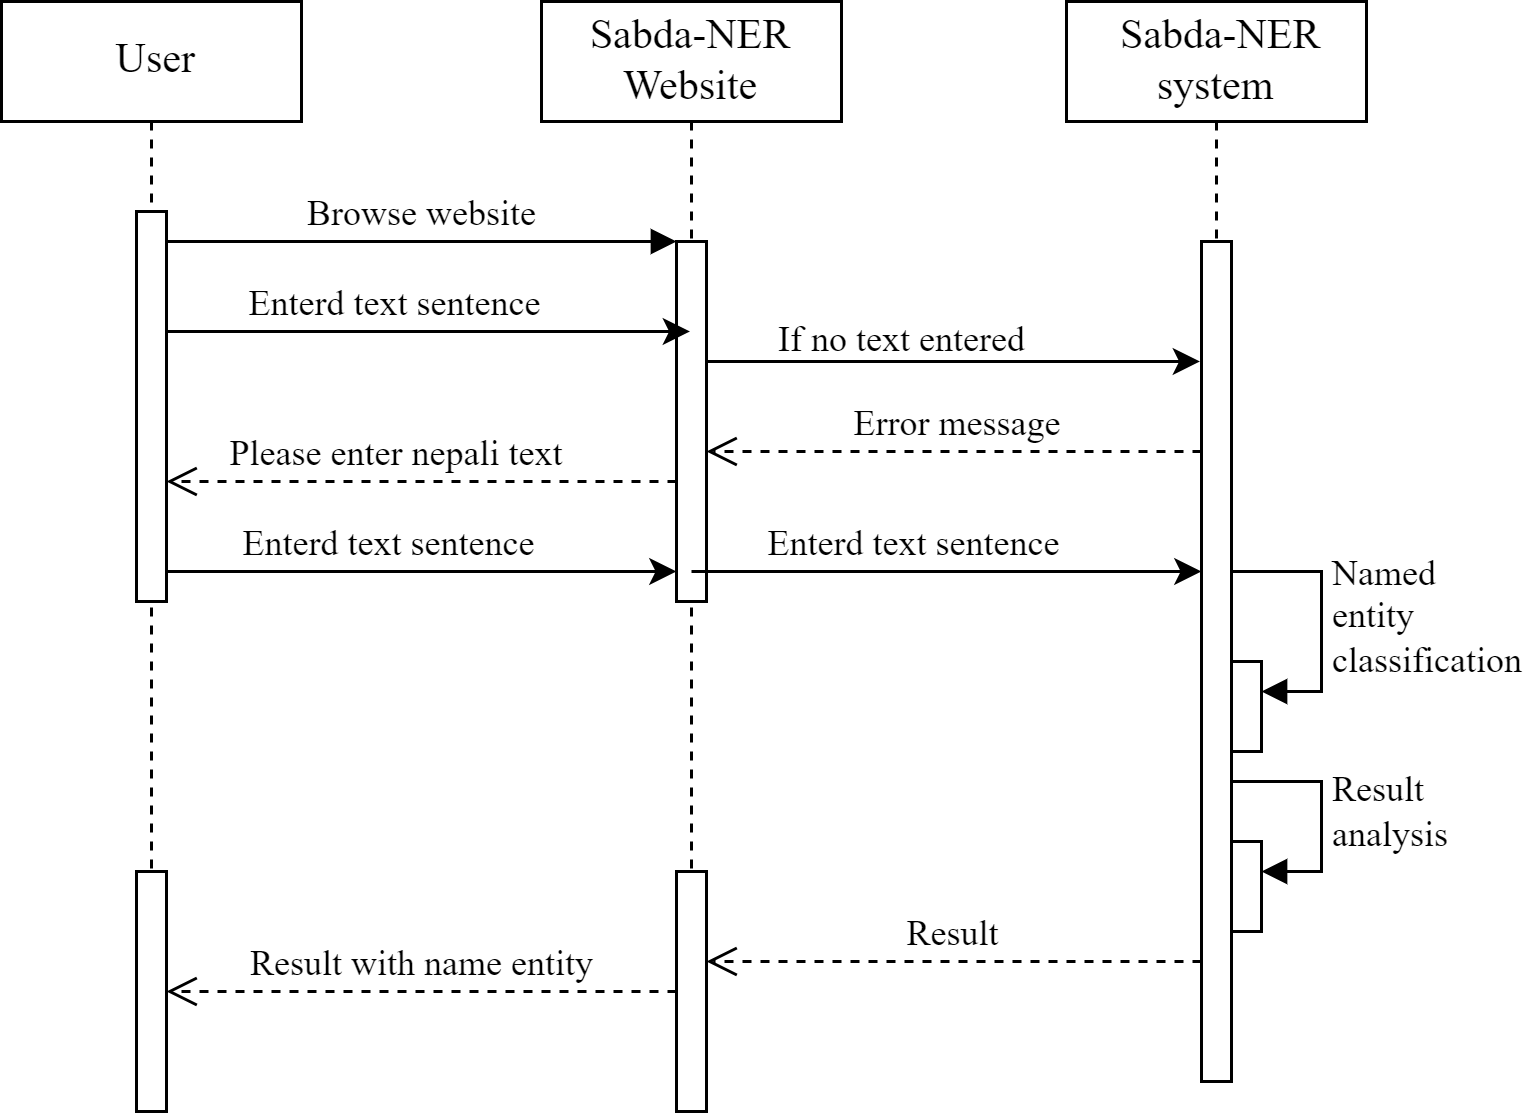
\includegraphics [scale=1.1]{img/systemBlock-etc/sabda ner sequence diagram.png}
\caption[ Sequence Diagram]{ Sequence Diagram}
% \label{fig:DisplaCy.png}

\end{figure}

 
The sequence diagram shows that the user initiates the process by accessing the system and providing their login credentials. The Server checks the login credentials and verifies the user’s identity. Once authenticated, the user proceeds to upload a Nepali to get the named entity information. Nepali text goes for preprocessing and feature extraction. Then processed data is fed into the NER model and is used to extract entities from the Nepali text. Lastly, users get information about different entities.\\


\\

\vspace{40pt} % Adjust the value as needed
\subsection{Data Flow Diagram}
\vspace{30pt} % Adjust the value as needed
\subsubsection{ Level 0 DFD}


\begin{figure}[H]
\centering
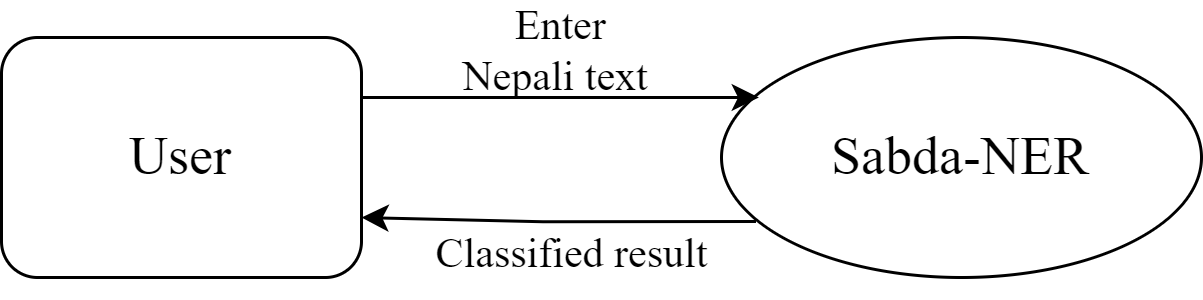
\includegraphics [scale=1]{img/systemBlock-etc/_dfd 0.png}
\caption[ Level 0 DFD]{ Level 0 DFD}
% \label{fig:DisplaCy.png}

\end{figure}

\vspace{30pt} % Adjust the value as needed
 
DFD level – 0 indicates the basic flow of data in the system.
\begin{itemize}
    \item User: User input to the system is uploading Nepali text.
    \item System: In the system, text data are processed, and the NER model gives the
named entity that are present in that text.
\end{itemize}

Hence, the data flow diagram indicates the visualization of the system with its input
feed to the system by the User.


\subsubsection{Level 1 DFD}

\begin{figure}[H]
\centering
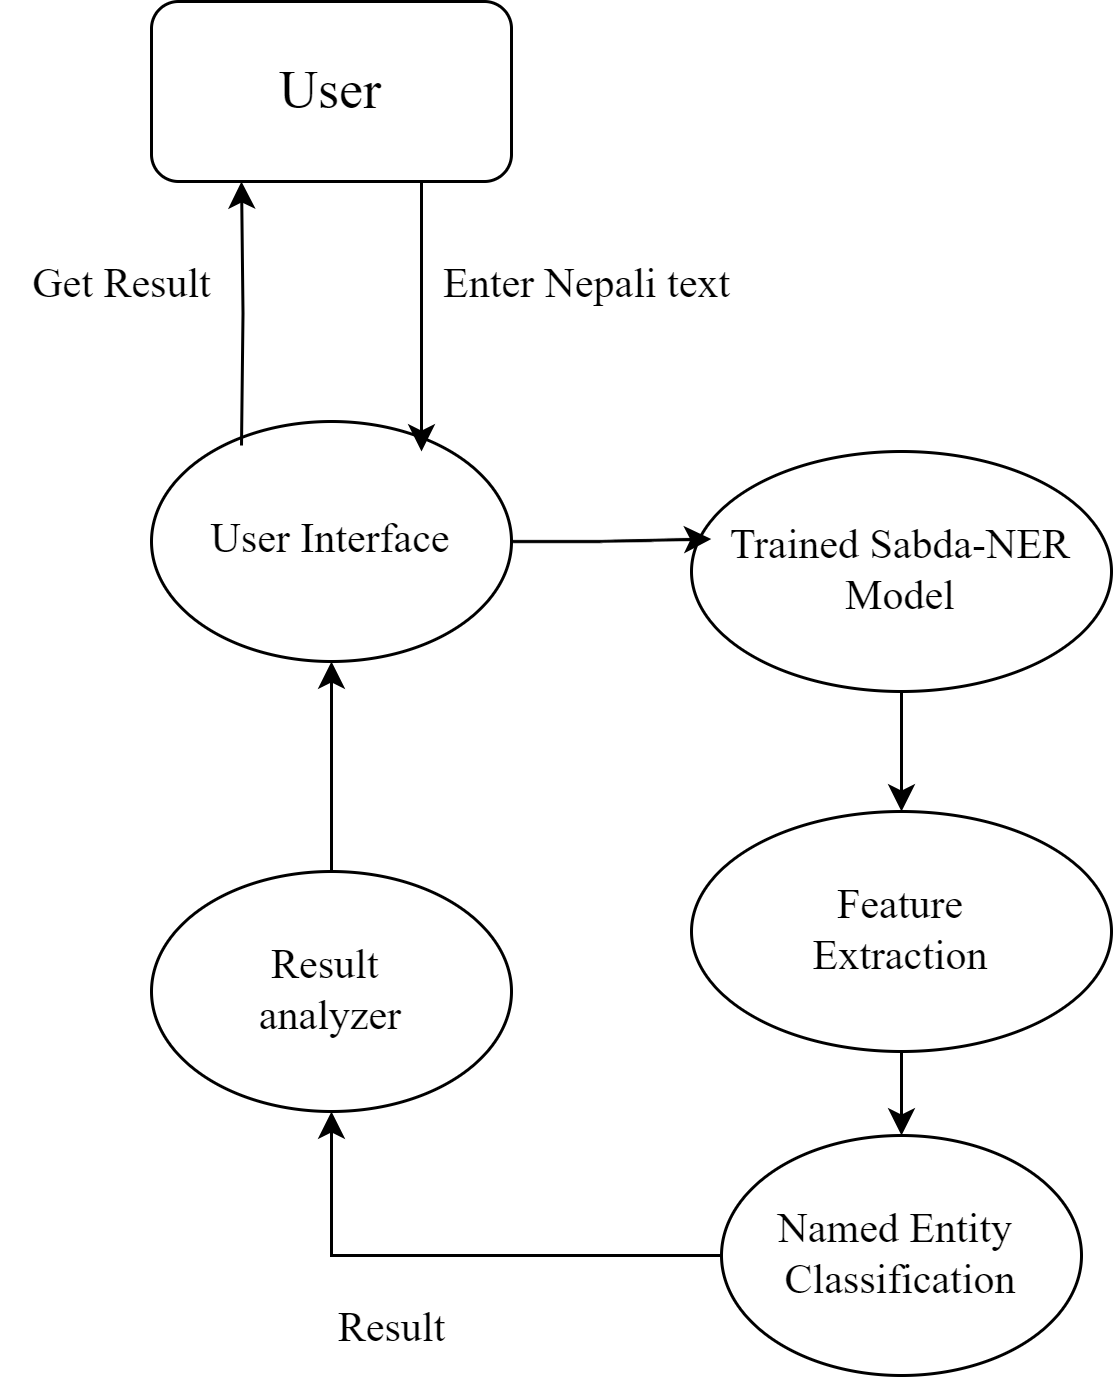
\includegraphics [scale=0.9]{img/systemBlock-etc/_dfd1.png}
\caption[ Level 1 DFD]{ Level 1 DFD}
% \label{fig:DisplaCy.png}

\end{figure}

 
DFD Level – 1 gives more in and out information about the system. Where the system
gives detailed information on the procedure taking place.

\subsection{Activity Diagram} 
\vspace{30pt} % Adjust the value as needed

  \begin{figure}[H]
\centering
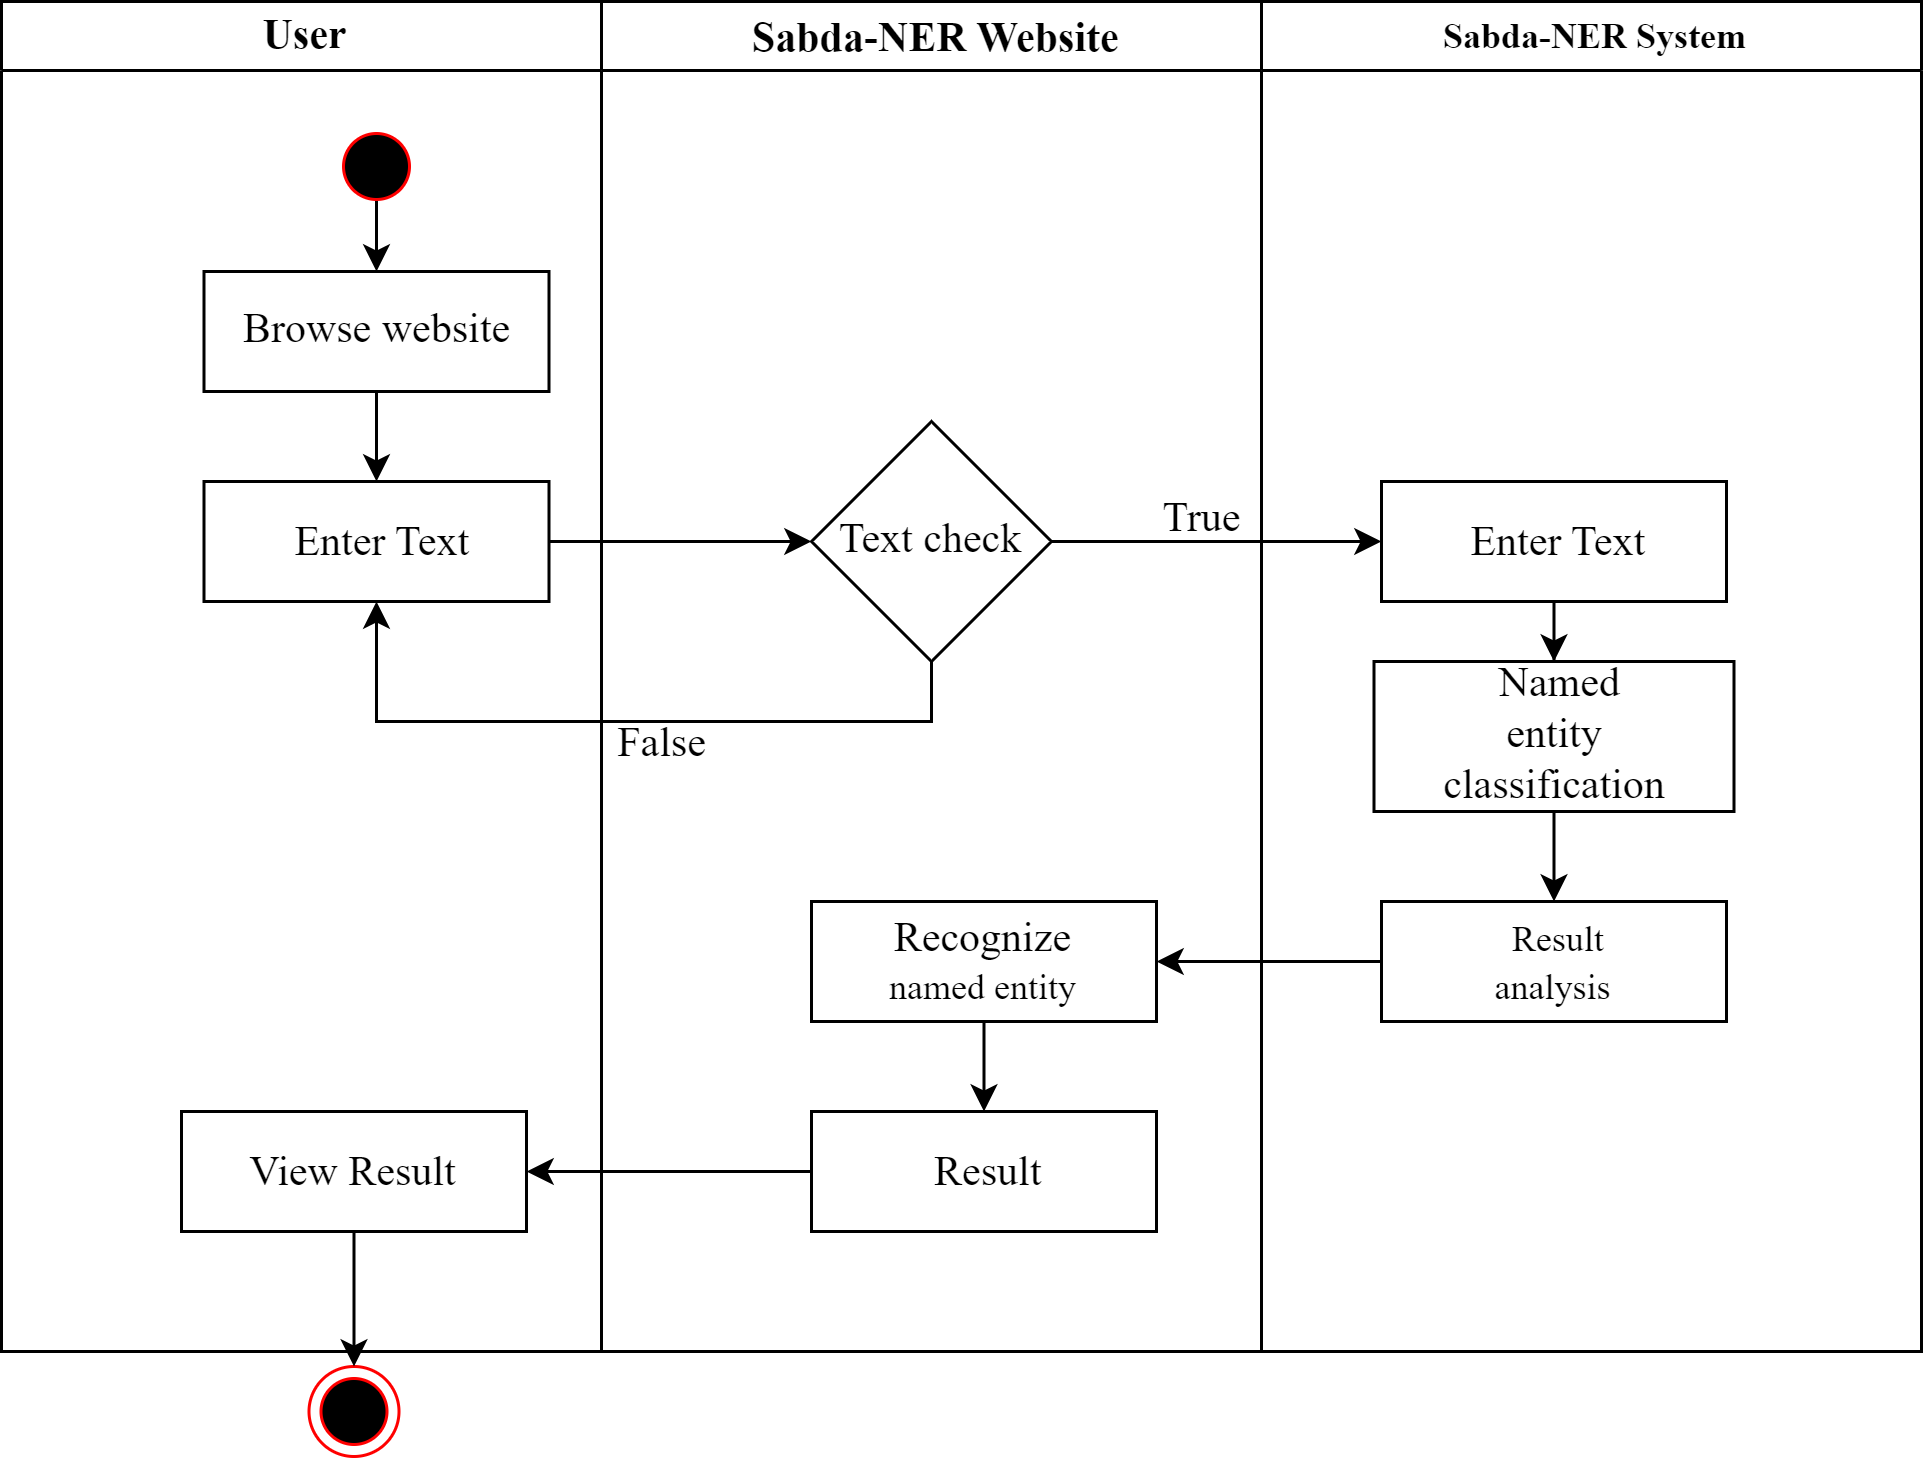
\includegraphics [scale=0.9]{img/systemBlock-etc/activity sabda ner.png}
\caption[ Activity Diagram]{Activity Diagram}
% \label{fig:DisplaCy.png}

\end{figure}

 
The activity diagram shows that the user initiates the process by accessing the browser and enter nepali text. The sabda-NER website checks whether the entered text is nepali or not. Once the text is checked the sabda-NER system classifies the named entities and the result is proveded through user interface.\\


% \begin{figure}[H]
% \centering
% 
\includegraphics[width=0.4\linewidth]{img/Graphics/TUlogo.png}
% \caption[System Block Diagram]{System Block Diagram}
% \label{fig:SystemBlockDiagram.png}

% \end{figure}

% Figure \ref{fig:SystemBlockDiagram.png}shows the intended system block diagram of the proposed system. 


%  \newpage

% \section{Dataset Collection}

% \begin{table}[H]
  
% \caption{Data Set Stats}
% \label{tab: Data Set Stats}
%     \centering
    
%     \begin{tabular}{|c|c|c|}
%         % \hline
%         % Column 1 & Column 2 & Column 3 \\
%         % \hline
%         % Row 1, Cell 1 & Row 1, Cell 2 & Row 1, Cell 3 \\
%         % Row 2, Cell 1 & Row 2, Cell 2 & Row 2, Cell 3 \\
%         % \hline
%     \end{tabular}
    
    
% \end{table}

% \begin{figure}[H]
% \centering
% 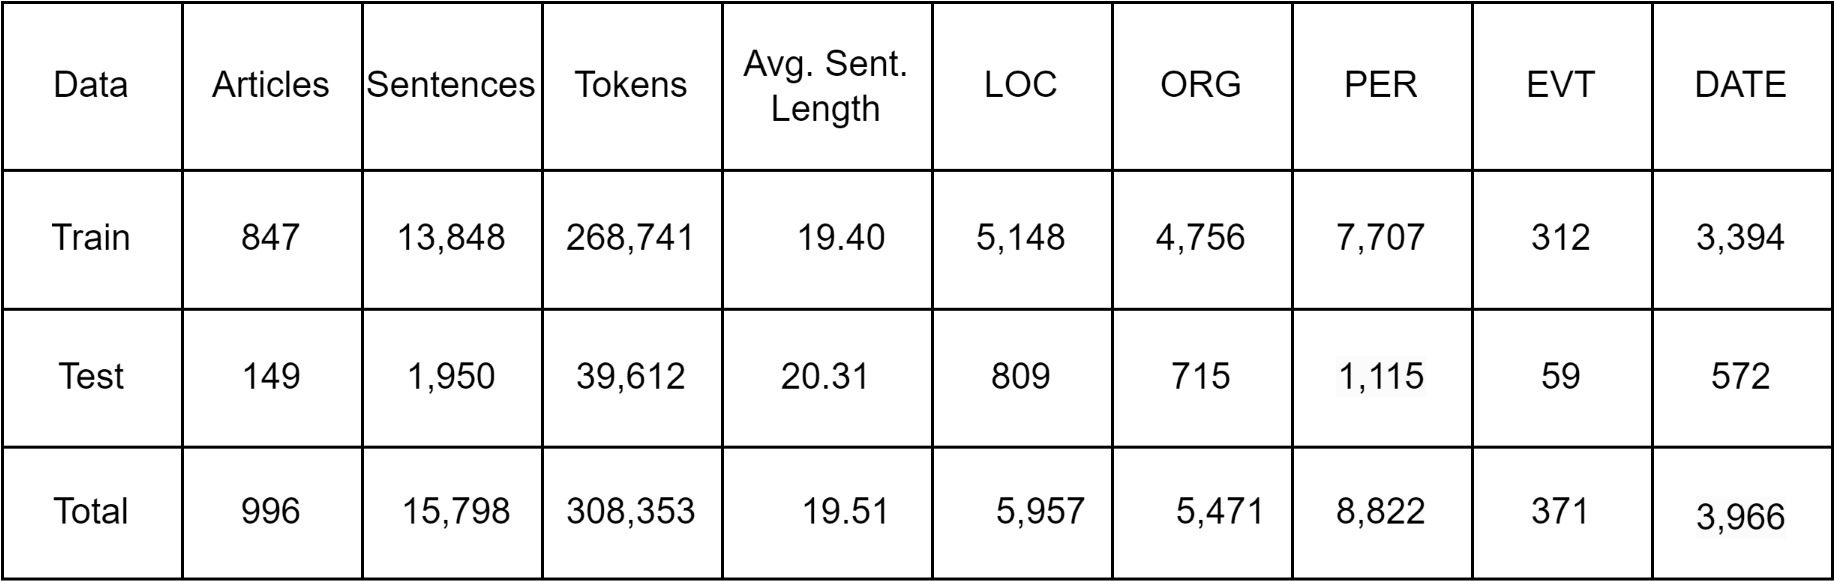
\includegraphics [scale=0.9]{img/Graphics/Data Set Stats.png}
% % \caption[  Data Set Stats]{ Data Set Stats}
% % \label{fig:DisplaCy.png}

% \end{figure}

% \textbf{Corpus Dataset} We have prepared human annotated Name Entity Recognition (NER) dataset for Nepali from the corpus data available at https://amitness.com/ml-datasets.\\
% \\
% We have taken Nepali News Corpus (i.e. from Nagarik and Setopati).We have used NLTK (a toolkit built for working with NLP) for tokenization.\\
% \\
% Our SABDA-NER covers three named entities – person’s, location's, and organization’s name during our research, we found Everest-NER from which we took reference. We will use the Everest-NER dataset for training our model for the first phase. Our SABDA-NER data will be used as a test dataset. From our initial research, we will be applying the BERT model for our NER project. Incoming challenges are further to be discussed.\cite{article2}


 
% \section{Description of Algorithm}
% \vspace{10pt} % Adjust the value as needed
% \subsection{Entities Set} 
% Natural Language Processing (NLP)’s named entity recognition (NER) sub-component seeks to identify the textual existence of entities that fall under a predetermined set of categories, such as “PERSON”, “LOCATION”, and “ORGANIZATION”.

% \subsection{Annotation Guidelines}
% We developed detailed annotation guidelines that cover entity types, variations, and potential challenges specific to the Nepali language. These guidelines will ensure consistent labeling during the annotation process.\\

 
% \begin{table}[H]
  
% \caption{ Annotation Guidelines}
% \label{tab:  Annotation Guidelines}
%     \centering
    
%     \begin{tabular}{|c|c|c|}
%         % \hline
%         % Column 1 & Column 2 & Column 3 \\
%         % \hline
%         % Row 1, Cell 1 & Row 1, Cell 2 & Row 1, Cell 3 \\
%         % Row 2, Cell 1 & Row 2, Cell 2 & Row 2, Cell 3 \\
%         % \hline
%     \end{tabular}
    
    
% \end{table}
% \begin{figure}[H]
% \centering
% 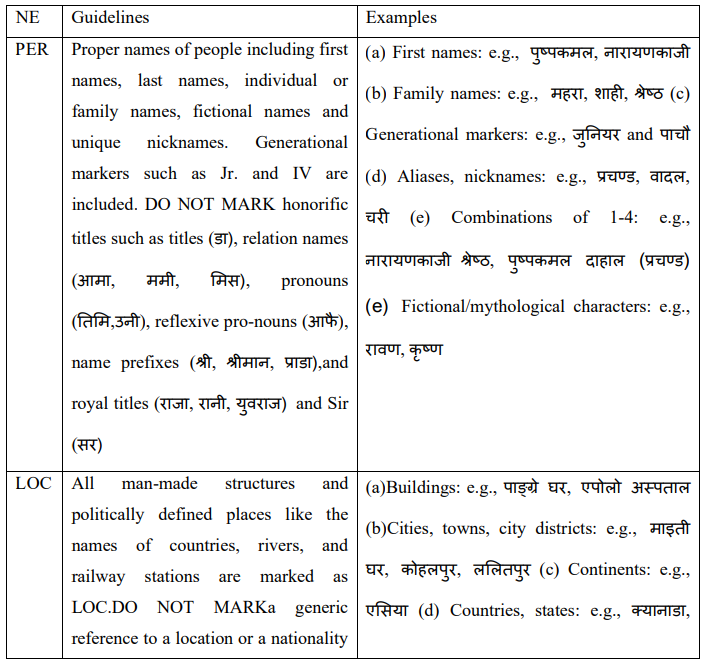
\includegraphics [scale=1.2]{img/Graphics/Annotation Guidelines1.png}
% % \caption[ Annotation Guidelines]{ Annotation Guidelines}
% % \label{fig:DisplaCy.png}

% \end{figure}
% \begin{figure}[H]
% \centering
% 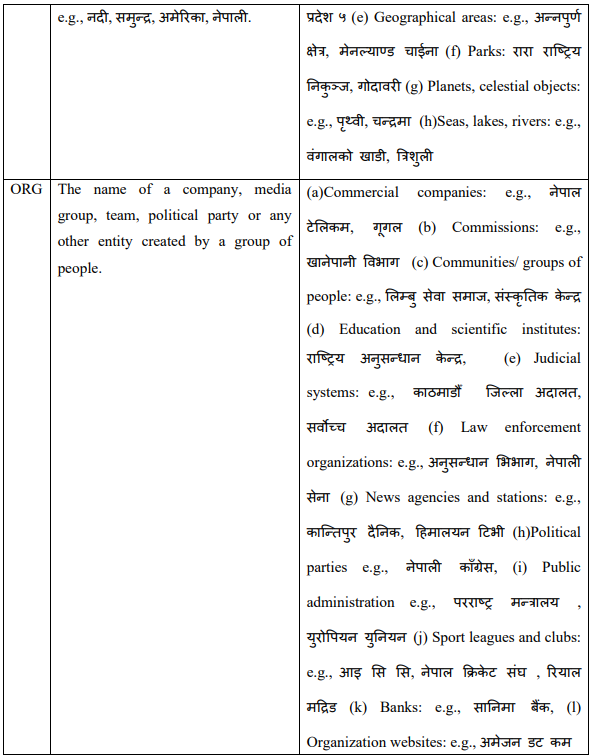
\includegraphics [scale=1.35]{img/Graphics/Annotation Guidelines2.png}
% % \caption[ Annotation Guidelines]{ Annotation Guidelines}
% % \label{fig:DisplaCy.png}

% \end{figure}



 
 
% \subsection{Model Selection}
% We fine-tuned pre-trained models that was trained for multi-lingual, the BERT-based-multilingual-cased model. To tailor it for Nepali, we began with a pre-trained model for a related language and fine-tuned it using our datasets.

% \subsection{Data Splitting}
% Splitting of annotated dataset into training, validation, and testing sets. A common split is 80-20, where 80\% of the data is used for training, and the rest is for validation, and we prepare few datasets to test the model.

% \subsection{Fine Tuning}
% As we utilized a pre-trained model, we proceeded to fine-tune it using our annotated Nepali dataset. Following the structure outlined in WikiANN, we tokenized the dataset into two sets—one for tokens and the other for NER tags. To adhere to the required format of .json files, we converted our annotated and cleaned dataset into train.json and validate.json files. These files were then used to train the model and validate its predictions.

% \subsection{Model Evaluation}
% We assessed our trained/fine-tuned model on the validation and testing datasets, employing metrics such as precision, recall, and F1-score. The model exhibited promising results, achieving an overall precision of approximately 0.98 across various validation and training datasets.

% \subsection{Model Deployment}
% We are working on deploying our model on a simple website, allowing users to enter the page, import their sentences, and extract the desired information.

% \newpage
% \section{Working Principle}
% \vspace{10pt} % Adjust the value as needed
% We have used News Corpus for preparing our dataset (Nepali News Corpus). News articles contain frequently used named entities. Articles have different domains like politics, sports, economics, art, society, and literature. The available corpus consists of text files. We used NLTK library to tokenize the text files. Preprocessing of data was done by removing punctuation marks and stop-words which helped to keep dataset clean. Later manual annotation was done to the dataset following the guidelines mentioned in data annotation.


 
% \begin{figure}[H]
% \centering
% 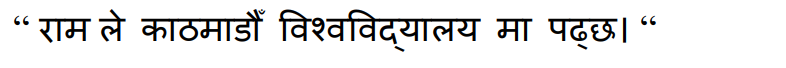
\includegraphics [scale=1.2]{img/workingPrinciple/ramle.png}
% % \caption[ Annotation Guidelines]{ Annotation Guidelines}
% % \label{fig:DisplaCy.png}

% \end{figure}


% The obtained tokens are annotated as following:

%   \begin{table}[H]
  
% \caption{ Label Dataset with annotation guideline}
% \label{tab:   Label Dataset with annotation guideline}
%     \centering
    
%     \begin{tabular}{|c|c|c|}
%         % \hline
%         % Column 1 & Column 2 & Column 3 \\
%         % \hline
%         % Row 1, Cell 1 & Row 1, Cell 2 & Row 1, Cell 3 \\
%         % Row 2, Cell 1 & Row 2, Cell 2 & Row 2, Cell 3 \\
%         % \hline
%     \end{tabular}
    
    
% \end{table}
 
% \begin{figure}[H]
% \centering
% 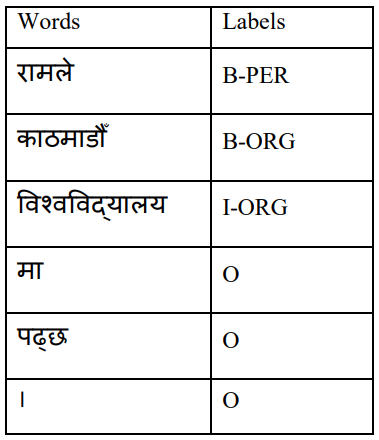
\includegraphics [scale=1.3]{img/workingPrinciple/ramle lebel.png}
% % \caption[ Annotation Guidelines]{ Annotation Guidelines}
% % \label{fig:DisplaCy.png}

% \end{figure}
 
% This data set is now all set for training. We have used ‘Pytorch’ library for loading datasets to training set into DataLoader. In PyTorch, when loading data using a DataLoader, it's crucial to convert text data into numbers for the model. This involves several steps for Named Entity Recognition (NER):

% \textbf{1.	Tokenization} : Split text into tokens.
%            Tokenized Sentence:
%            \begin{figure}[H]
% \centering
% 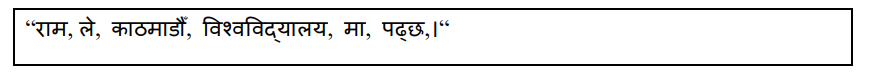
\includegraphics [scale=1]{img/workingPrinciple/ramle ku.png}
% % \caption[ Annotation Guidelines]{ Annotation Guidelines}
% % \label{fig:DisplaCy.png}

% \end{figure}
 
%            Labels:
           
% \begin{figure}[H]
% \centering
% 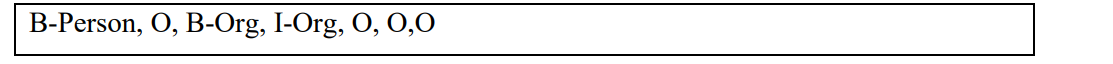
\includegraphics [scale=0.8]{img/workingPrinciple/org.png}
% % \caption[ Annotation Guidelines]{ Annotation Guidelines}
% % \label{fig:DisplaCy.png}

% \end{figure}
 
% \textbf{2.	Token-to-ID Mapping} : Convert tokens to numbers.
          
% Tokenized Sentence:

% \begin{figure}[H]
% \centering
% 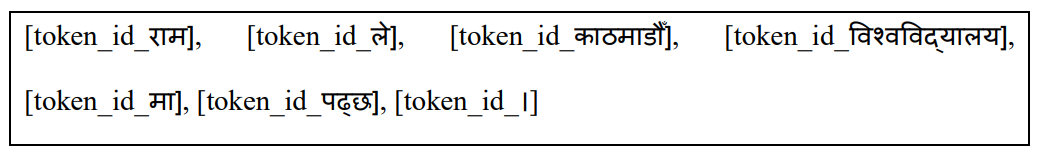
\includegraphics [scale=0.8]{img/workingPrinciple/token.png}
% % \caption[ Annotation Guidelines]{ Annotation Guidelines}
% % \label{fig:DisplaCy.png}

% \end{figure}
 
% \textbf{3.	Padding} : Make all sequences the same length.

% \begin{figure}[H]
% \centering
% 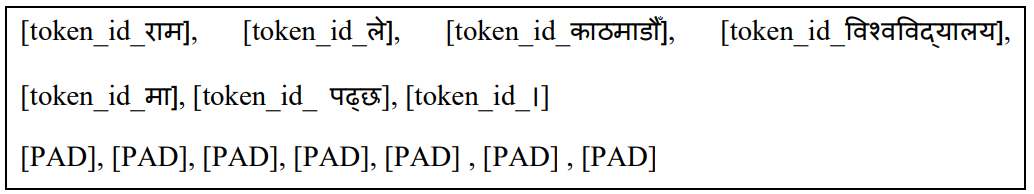
\includegraphics [scale=0.8]{img/workingPrinciple/token pad.png}
% % \caption[ Annotation Guidelines]{ Annotation Guidelines}
% % \label{fig:DisplaCy.png}

% \end{figure}
 
% \textbf{4.	Label Encoding} : Turn NER labels into numbers.
% \begin{figure}[H]
% \centering
% 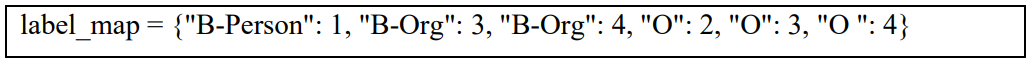
\includegraphics [scale=0.8]{img/workingPrinciple/lebelmap.png}
% % \caption[ Annotation Guidelines]{ Annotation Guidelines}
% % \label{fig:DisplaCy.png}

% \end{figure}
 
%  Encoded Labels:  
%  \begin{figure}[H]
% \centering
% 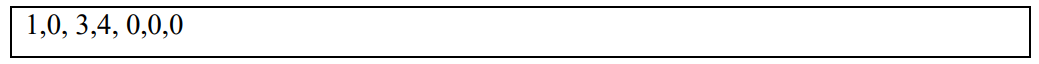
\includegraphics [scale=0.8]{img/workingPrinciple/0101.png}
% % \caption[ Annotation Guidelines]{ Annotation Guidelines}
% % \label{fig:DisplaCy.png}

% \end{figure}
 
% Data Loader of huggingface datasets enable efficient use of transformers as well as neural networks. They streamline data processing and enhance model training for tasks like NER. 
% After properly loading our dataset in the DATA loader we will be using BERT-based-multilingual pre-trained model (Initial Phase) and also refer other models to train and fine-tune our model. 




% \newpage
% \textbf{}\section{Verification and Validation}
% \vspace{10pt}
% In google colab, we used hardware accelerator T4 GPU to train our model.
% We imported seqeval library to calculate the overall precision, overall recall. And overall f1 score. 
% Seqeval is a Python library for sequence labeling evaluation commonly used to evaluate the performance of models that perform sequence labeling tasks like NER models.
% It provides functions to compute common evaluation metrics such as precision, recall and F1 score for sequence labelling tasks.
% These metrics are standard in the field of natural language processing (NLP) and machine learning for evaluating the performance.\\

% In the context of evaluation metrics for classification tasks, such as in machine learning or natural language processing, precision, recall, and F1 score are commonly used metrics to assess the performance of a model.

% \textbf{Overall Precision} :
%    Precision is the ratio of true positive predictions to the total number of positive predictions (true positives + false positives). It measures the accuracy of positive predictions made by the model.
    

%     \begin{equation}
% \text{Precision} = \frac{\text{True Positives}}{\text{True Positives + False Positives}}
% \end{equation}


% \textbf{Overall Recall} :
%    Recall, also known as sensitivity or true positive rate, is the ratio of true positive predictions to the total number of actual positives (true positives + false negatives). It measures the ability of the model to capture all the positive instances.
   
%    \begin{equation}
%         \text{Recall} = \frac{\text{True Positives}}{\text{True Positives + False Negatives}} 
%    \end{equation}
  

% \textbf{Overall F1 Score} :
%    The F1 score is the harmonic mean of precision and recall, providing a balanced measure that considers both false positives and false negatives. It ranges from 0 to 1, where higher values indicate better model performance.
%    \begin{equation}
%         F1 \text{ Score} = \frac{2 \times \text{Precision} \times \text{Recall}}{\text{Precision + Recall}} 
%    \end{equation}
  

% The terms "overall" in precision, recall, and F1 score typically imply that these metrics are calculated considering all classes or categories in a multi-class classification problem. These metrics provide a comprehensive evaluation of a model's performance across all classes rather than focusing on individual classes.



